\documentclass[a4paper, 12pt, addpoints]{exam}
\usepackage{IfbaListas}
%==============================================================
\NumList{5} %NÚMERO DA LISTA
\Assunto{Combinatória}
%==============================================================
%=========================================================
%------------Cabeçalho e rodapé 
%=========================================================
\pagestyle{headandfoot}%{head}%empty
\firstpageheader{}{}{}
\runningheader{\disciplina}{}{Lista \numlist: \assunto}
\runningheadrule
% \copyright \professor
\firstpagefooter{}{}{Pag. \thepage\ de \numpages}
%\iflastpage{Outros templates em \href{http://gg.gg/profwaldexsantos}{gg.gg/profwaldexsantos}
\runningfooter{}{}{Pag. \thepage\ de \numpages}
\runningfootrule
%===============================================================
%INFORMAÇÕES SOBRE A AVALIAÇÃO
\nomeInst{Instituto Federal da Piauí}
\logoInst{
\includegraphics[scale=0.17]{Figs/IFPIPicosVertical.png}}
\Campus{Picos} %PARA ENSINO FUNDAMENTAL OU MÉDIO-COMENTE ESTA LINHA COM %
\nomeCurso{Análise e Desenvolvimento de Sistemas} %Se não for curso superior, basta comentar esta linha ou deixar em branco
\nomeDisciplina{Matemática Computacional}
\Semestre{1}
\nomeProfessor{Rogerio Figueredo de Sousa}
\Aluno{}
\matriculaAluno{}
%===============================================================
 %CARREGA AS INFORMAÇÕES GERAIS DO PROFESSOR, ESCOLA ETC
%==============================================================

%COMEÇO DO DOCUMENTO
\begin{document}
\info\vspace{-1 cm} %Imprime as informações do cabeçalho programada no pacote 
% inicia a gravacao da resposta no arquivo "ans" cujo nome externo é gabarito 
\Opensolutionfile{ans}[Gabarito]
%*****************************************************************************
\begin{questions}%COMEÇA O AMBIENTE DE QUESTÕES
  \question De quantas maneiras as letras da palavra CURSO podem ser permutadas?
  
  \begin{resp}~

    Cada anagrama de CURSO nada mais é que uma ordenação das letras C, U, R, S, O. Assim, o número de anagramas de CURSO é $P_5 = 5! = 5 . 4 . 3 . 2 .  1 = 120$.
  \end{resp}

  \question Um cubo de madeira tem as faces pintadas de cores diferentes. De  quantos modos podem ser gravados números de 1 a 6 sobre cada uma das faces?

  \begin{resp}~

    Devemos colocar seis cores em seis lugares. Logo, a resposta é $P_6 = 6! = 6.5 . 4 . 3 . 2 . 1 = 720$.
  \end{resp}

  \question Considere 4 cidades A, B, C e D. Ana e João pensam fazer um passeio pelas 4 cidades, passando por cada uma delas apenas uma vez.

  \begin{enumerate}[a)]
    \item Se eles podem começar por qualquer cidade e terminar em qualquer cidade, quantos trajetos são possíveis?
    \item Se eles devem começar pela cidade A, quantos caminhos são possíveis? 
  \end{enumerate}

  \begin{resp}~

    \begin{enumerate}[a)]
      \item $4! = 4 . 3 . 2 . 1 = 24$ trajetos possíveis, pois cada passeio corresponde a uma forma diferente de visitar a cidade.
      \item $3! = 3 . 2 . 1 = 6$, pois a cidade A é fixa.
    \end{enumerate}
  \end{resp}
  
  
\question De quantos modos é possível colocar em uma prateleira 5 livros distintos de matemática, 3 diferentes de física e 2 diferentes de inglês?

\begin{resp}~

  Como não existe restrição, podemos ordenar os livros de qualquer maneira.Como temos ao todo 10 livros, daí a resposta é $P_10 = 10! = 3628800$.
\end{resp}

\question Quantos são os anagramas da palavra ÂNGULO que:

\begin{enumerate}[a)]
    \item Começam com vogal?
    \item Começam e terminam por vogal?
    \item Não têm juntas as letras A e N?
\end{enumerate}

\begin{resp}~

  \begin{enumerate}[a)]
    \item A vogal inicial pode ser escolhida de 3 maneiras, e as letras restantes podem ser arrumadas de $P_5 = 5!$ maneiras. Logo, pelo princípio multiplicativo, a resposta é $3 . 5! = 360$.
    \item A vogal inicial pode ser escolhida de 3 maneiras, a vogal final de 2 maneiras e as 4 letras restantes podem ser arrumadas entre essas duas vogais de $P_4 = 4!$ modos. Logo, a resposta é $3 . 2 . 4! = 3 . 2 . 4 . 3 . 2 . 1 = 144$. Observemos que obtemos o mesmo resultado se começamos com a possibilidade da última letra, depois continuamos coma as possi-
    bilidades da primeira letra e finalmente as quatro letras restantes.
    \item O número de anagramas com 6 letras é $P_6 = 6! = 720$. O número de maneiras de ordenar 6 letras de modo que 2 letras, A e N , fiquem juntas é $2 . 5!$, pois para formar um anagrama, devemos inicialmente decidir em que ordem se colocarão \textit{A} e \textit{N} (\textit{AN} ou \textit{NA}), e, em seguida, formar o anagrama com 5 letras. Portanto a resposta é $6! - 2.5! = 720 - 240 = 480$.

  \end{enumerate}
\end{resp}



\question De quantos modos 5 meninas e 5 meninos podem formar uma roda de
ciranda de modo que pessoas do mesmo sexo não fiquem juntas?

\begin{resp}~

  Existe uma permutação circular com as 5 meninas, isto é, $(PC)_5 = 4!$ modos de formar uma roda com as meninas. Depois disso, os 5 meninos devem ser postos nos lugares entre as meninas, o que pode ser feito de $5!$ modos. A resposta é $4!5! = 2880$.
\end{resp}

\question De quantos modos 4 casais podem formar uma roda de ciranda de modo
que cada homem permaneça ao lado da sua mulher e que pessoas do
mesmo sexo não fiquem juntas?

\begin{resp}~

  Existe uma permutação circular com os 4 homens, isto é, $(PC)_4 = 3!$ modos de formar uma roda como os 4 homens. Depois disso, há dois modos de pôr as esposas na roda: à direita ou à esquerda de seus maridos. A resposta é $2 . 3! = 12$.
\end{resp}

\question De quantos modos 5 mulheres e 6 homens podem formar uma roda de
ciranda de modo que as mulheres permaneçam juntas?

\begin{resp}~

  Podemos formar uma roda com os homens de $(PC)_6 = 5!$ modos. Depois, devemos escolher um dos 6 espaços entre os homens (o que pode ser feito de 6 modos) para aí colocarmos todas as mulheres. Finalmente, devemos decidir em que ordem as 5 mulheres se colocarão nesse espaço ($5!$ modos). A resposta é $5!6 . 5! = 5!6! == 86400$.
\end{resp}

\question Em uma comissão de 10 professores devem ser escolhidos um coordenador e um subcoordenador. De quantas maneiras eles podem ser escolhidos?

\begin{resp}~

  Observemos que temos 10 professores e devemos fazer 2 escolhas, coordenador e subcoordenador (importa a ordem emq ue são considerados). Portanto, esta questão tem as características dos arranjos simples, onde o número total de elementos diferentes considerados são 10 e cada escolha de 2 professores corresponde a uma possibilidade. Então, o número de maneiras emq ue eles podem ser escolhidos é $A(10,2) = \frac{10!}{(10-2)!} = 10 . 9 = 900$
\end{resp}

\question De quantas maneiras 4 amigos entre 10 podem se colocar em uma foto?

\begin{resp}~

  Observemos que, escolhidos 4 amigos dentre 10, a ordem como eles podem aparecer na foto dá lugar a possibilidades diferentes. Portanto, o número de maneiras como 4 amigos dentre 10 podem se colocar em uma foto corresponde a arranjos simples, $A(10,4) = \frac{10!}{6!}$
\end{resp}

\question Quantos tipos de bilhetes especificando a origem e o destino têm uma compania aérea que une 7 cidades?

\begin{resp}~

  42
\end{resp}

\question Considere os números de 3 algarismos distintos formados com os dígitos 2, 3, 5, 8, e 9.

    \begin{enumerate}[a)]
        \item Quantos são estes números?
        \item Quantos são menores do que 800?
        \item Quantos são múltiplos de 5?
        \item Quantos são pares?
        \item Quantos são ímpares?
    \end{enumerate}

    \begin{resp}~

      \begin{enumerate}[a)]
        \item O número de 3 algarismos distintos formados com os dígitos 2,3,5,8 e 9 é $A(5,3) = 60$
        \item Como os números devem ser menores do que 800, significa que o primeiro algarismo (centena) não pode começar nem com 8 nem com 9. Portanto, para esta posição, temos 3 possibilidades. Escolhida uma possibilidade para a primeira posição, sobram 4 números para as outras 2 posições (dezena e unidade), isto é, temos $A(4,2)$ possibilidades. Então, pelo princípio multiplicativo, temos que a quantidade de números de 3 algarismos menores de 800 que podem ser formados com os números 2,3,5,8 e 9 é $ 3. A(4,2) = 36$
        \item Com os dígitos dados, os únicos números múltiplos de 5 são os que finalizam em 5. Portanto, restam para as outras duas posições (centenas e dezenas) os números 2,3,8 e 9 tomados 2 a 2. Logo, os múltiplos de 5 são $A(4,2) = 12$.
        \item Os números pares são $2.A(4,2) = 24$
        \item Os números ímpares são $3.A(4,2) = 36$
    \end{enumerate}
    \end{resp}

\question Quantas são as palavras de 5 letras distintas de um alfabeto de 26 letras nas quais a letra \textbf{A} aparece mas não é a letra inicial da palavra?

\begin{resp}~

  Para a letra inicial das palavras de 5 letras distintas temos 25 possibilidades pois não pode ser a letra $A$.

Fixada a primeira letra, a letra $A$ pode ocupar na palavra 4 posições diferentes.

Fixada a primeira letra e a posição de $A$ na palavra de 5 letras, restam 3 posições que podem ser preenchidas com 24 letras diferentes do alfabeto. Então, dadas 24 letras, o número de possibilidades de formar anagramas de 3 letras distintas é $A(24, 3) = \frac{24!}{21!}$.

Portanto, considerando as possibilidades para a letra inicial, para a posição de $A$ e para as 3 letras restantes e usando o princípio multiplicativo, concluímos que o número de palavras de 5 letras distintas de um alfabeto de 26 letras nas quais a letra $A$ figura mas não é a letra inicial da palavra é $25 \cdot 4 \cdot \frac{24!}{21!} = 4 \cdot \frac{25!}{21!}$.

\end{resp}

\question Quantos números de 3 e 4 algarismos distintos e maiores do que 300 podem ser formados com os algarismos 0, 1, 3, 5 e 7?

\begin{resp}~

  Começamos calculando a quantidade de números de 3 algarismos distintos e maiores do que 300 formados com 0, 1, 3, 5 e 7. Observemos que para o primeiro dígito (centena) temos 3 possibilidades $(3, 5 \text{ ou } 7)$. Para as duas posições restantes temos $A(4, 2)$ possibilidades (incluímos 0 e 1). Portanto, devido ao princípio multiplicativo, neste caso temos $3A(4, 2) = 36$ modos diferentes.

Agora calculamos a quantidade de números com 4 algarismos distintos formados com 0, 1, 3, 5 e 7. Para a primeira posição temos 4 maneiras $(1, 3, 5 \text{ ou } 7)$. Fixado um número na primeira posição, temos $A(4, 3)$ possibilidades, pois também devemos considerar o 0. Logo, neste caso, usando o princípio multiplicativo temos $4A(4, 3) = 96$ possibilidades.

Finalmente, usando o princípio aditivo, obtemos que a quantidade de números de 3 e 4 algarismos distintos e maiores do que 300 que podem ser formados com os algarismos 0, 1, 3, 5 e 7 é $36 + 96 = 132$.

\end{resp}

\question Quantos são os números de 5 algarismos distintos na base 10:

\begin{enumerate}[a)]
    \item Nos quais o algarismo 2 aparece?
    \item Nos quais o algarismo 2 não aparece?
\end{enumerate}

\begin{resp}~

  \begin{enumerate}[a)]
    \item Separamos o raciocínio em duas partes. Na primeira consideramos que o 2 está na primeira posição e na segunda etapa consideramos que o 2 não aparece na primeira posição.

    Na primeira situação, temos de escolher 4 algarismos distintos dentre 9 dígitos. Portanto, os números de 5 algarismos distintos na base 10 que começam com 2 são $A(9, 4) = 3024$.
    
    Na segunda parte, os números podem começar de 8 formas diferentes (estão excluídos 0 e 2). Logo, uma das 4 posições restantes deve ser ocupada por 2. Fixados o primeiro dígito do número e a posição do 2, restam 3 lugares a serem preenchidos com 8 dígitos diferentes que pode ser feito de $A(8, 3)$ modos diferentes. Portanto, neste caso, pelo princípio multiplicativo temos $8 \cdot 4 \cdot A(8, 3) = 10752$ possibilidades.
    
    Os números de 5 algarismos distintos na base 10 nos quais o algarismo 2 figura é a união do conjunto de números de 5 algarismos distintos na base 10 que começam com 2 e do conjunto de números de 5 algarismos distintos na base 10 que não começam com 2, que são disjuntos. Logo, pelo princípio aditivo, temos que a quantidade dos números de 5 algarismos distintos na base 10 nos quais o algarismo 2 figura é $9 \cdot \frac{8!}{5!} + 32 \cdot \frac{8!}{5!} = 13776$.

    \item O problema é equivalente a encontrar a quantidade de números de 5 algarismos distintos formados com os algarismos 0, 1, 3, 4, 5, 6, 7, 8, 9, que corresponde a $8.A(8,4) = 8.\frac{8!}{4!}$.
    
  \end{enumerate}
\end{resp}


\question Um estudante recebe uma prova contendo 6 questões. Ele deve escolher
4 para resolver. De quantas maneiras diferentes ele pode fazer essa escolha?

\begin{resp}~

  O estudante deve selecionar um grupo de 4 num total de 6 questões.

  Note que a ordem da resolução das questões não é importante: Resolvendo em ordem 1, 2, 3 e 4 ou, resolvendo 4, 3, 2 e 1 nesta ordem, de qualquer forma o aluno terá resolvido as mesmas questões.

  Portanto, o aluno pode fazer esta escolha de $C(6,4) = 15 maneiras$.
\end{resp}

\question Uma turma de calouros tem 15 rapazes e 10 moças. Devem escolher 2
representantes. De quantas maneiras eles podem ser escolhidos?

\begin{resp}

  A turma tem 25 alunos, dentre estes podemos escolher 2 alunos de $C(25,2) = 300$ maneiras.
\end{resp}

\question De quantos modos 5 meninas e 3 meninos podem ser divididos em 2
grupos de 4 crianças de forma tal que cada grupo inclua pelo menos 1
menino?

\begin{resp}
  
  Nessa questão adotaremos o seguinte raciocínio: Ao invés de contar o que é pedido no problema, contaremos seu complementar, subtrairemos este resultado do total e assim obteremos o número desejado.

O conjunto complementar é calculado em relação ao conjunto formado pelas possíveis divisões de 8 crianças em 2 grupos de 4 (conjunto universo).

Note que o único jeito de partirmos as crianças em 2 grupos de 4, de tal forma que algum desse grupos não tenha pelo menos um menino, é distribuir as crianças em um grupo com 4 meninas e outro com 3 meninos e uma menina.

Podemos dividir 8 crianças em 2 grupos de 4 crianças da seguinte forma: Escolhemos 4 crianças para ficar num grupo, para isso temos $C(8,4)$ maneiras e as restantes colocamos no outro grupo. Note que uma distribuição fixa é contada mais de uma vez, pois se enumerarmos as crianças de 1 a 8, o agrupamento $\{1,2,3,4\}$, $\{5,6,7,8\}$, onde o primeiro grupo representa o grupo formado pela escolha de 4 entre 8 crianças e o segundo pelas crianças restantes é equivalente a $\{5,6,7,8\}, \{1,2,3,4\}$. Precisamos portanto dividir o total pelo número de permutações entre os 2 grupos que é $P_2 = 2$. Logo, podemos distribuir 8 crianças em 2 grupos de 4 de $\frac{C(8,4)}{P_2} = \frac{70}{2} = 35 \text{ maneiras}.$

Para dividir as crianças em grupos onde um dos grupos não tenha nenhum menino, devemos colocar os 3 meninos num único grupo, depois temos $C(5,1)$ maneiras para determinar qual das meninas fará parte do grupo onde estão os 3 meninos. As meninas restantes irão compor o outro grupo.

O total de grupos com pelo menos 1 menino é $\frac{C(8,4)}{P_2} - C(5,1) = 35 - 5 = 30.$


\end{resp}

\question Uma comissão formada por 3 homens e 3 mulheres deve ser escolhida
em um grupo de 8 homens e 5 mulheres.

\begin{enumerate}[a)]
    \item Quantas comissões podem ser formadas?
    \item Qual seria a resposta se um dos homens não aceitasse participar da comissão se nela estivesse determinada mulher?
\end{enumerate}

\begin{resp}~

  \begin{enumerate}[a)]
    \item Para compor a comissão devemos escolher 3 em um grupo de 8 homens, o que nos dá um total de $C(8,3) = 56 maneiras$. Analogamente para as mulheres temos $C(5,3) = 10 maneiras$. Portanto, pelo princípio multiplicativo temos $C(8,3) . C(5,3) = 56 . 10 = 560$ comissões distintas.
    \item Dividiremos as comissões em dois grupos: Comissões onde se encontra a determinada mulher e comissões onde a mesma não se encontra.

    Contando o número de comissões onde a mulher se encontra, temos $C(4,2) = 6$ maneiras de preencher as outras vagas destinadas a mulheres, e como não poderemos contar com um dos homens, temos $C(7,3) = 35$ maneiras de selecionar os homens que vão compor a comissão. Portanto, pelo princípio multiplicativo, temos $C(4,2) \cdot C(7,3) = 210$ comissões distintas.
    
    Sabendo que a determinada mulher não se encontra na comissão, temos $C(4,3) = 4$ formas de escolher as 3 mulheres e $C(8,3) = 56$ maneiras de escolher os 3 homens. Portanto, pelo princípio multiplicativo, temos $C(4,3) \cdot C(8,3) = 224$ comissões distintas.
    
    Logo, pelo princípio aditivo, podemos montar um total de $210 + 224 = 434$ comissões distintas.
    
\end{enumerate}
\end{resp}

\question Para a seleção brasileira foram convocados 2 goleiros, 6 zagueiros, 7
meios de campo e 4 atacantes. De quantos modos é possível escalar a
seleção com 1 goleiro, 4 zagueiros, 4 meios de campo e 2 atacantes?

\begin{resp}
  
  Podemos escalar o goleiro de $C(2,1) = 2$ maneiras, os zagueiros de $C(6,4) = 15$ formas, os meio de campo de $C(7,4) = 35$ maneiras e os atacantes de $C(4,2) = 6$ maneiras. Pelo princípio multiplicativo, podemos montar o time de $C(2,1) . C(6,4) . C(7,4) . C(4,2) = 2 . 15 . 35 . 6 = 6300$ maneiras.
\end{resp}

\question Considere 3 vogais diferentes (incluindo o A) e 7 consoantes diferentes (incluindo o B).

\begin{enumerate}[a)]
    \item Quantas anagramas de 5 letras diferentes podem ser formados com 3 consoantes e 2 vogais?
    \item Quantas começam com A?
\end{enumerate}

\begin{resp}~

  \begin{enumerate}[a)]
    \item Inicialmente devemos selecionar quais vogais irão ser utilizadas nos anagramas, podemos fazer isso de $C(3,2) = 3$ formas. Agora determinamos as posições destas vogais no anagrama, podemos fazer isto de $A(5,2) = 20$ maneiras. Pelo princípio multiplicativo, temos $C(3,2)A(5,2) = 60$ formas de selecionar e alocar as vogais.

    Em relação às consoantes, devemos inicialmente selecionar 3, podemos fazer isto de $C(7,3) = 35$ maneiras. Depois temos que distribuir as consoantes escolhidas nas 3 posições restantes, isto pode ser feito de $P_3 = 6$ maneiras. Pelo princípio multiplicativo, temos $C(7,3)P_3 = 210$ formas de selecionar e alocar as vogais.
    
    Logo, pelo princípio multiplicativo, o número total de anagramas é $60\cdot210 = 12600$.
    
    \item Fixemos a vogal A no início da palavra, devemos agora preencher o anagrama das letras à direita do A, isto é, um anagrama de 4 letras onde devemos usar uma vogal e 3 consoantes. O procedimento adotado será análogo ao do item anterior.
    
    Primeiro selecionamos qual é a outra vogal a ser utilizada no anagrama (observe que não podemos mais usar a vogal A), podemos fazer isso de $C(2,1) = 2$ formas. Agora determinamos a posição desta vogal no anagrama, podemos fazer isto de $A(4,1) = 4$ maneiras. Pelo princípio multiplicativo, temos $C(2,1)A(4,1) = 8$ formas de selecionar e alocar as vogais.
    
    Para as consoantes, devemos inicialmente selecionar 3, podemos fazer isto de $C(7,3) = 35$ maneiras. Depois temos que distribuir as consoantes escolhidas nas 3 posições restantes, isto pode ser feito de $P_3 = 6$ maneiras. Pelo princípio multiplicativo, temos $C(7,3)P_3 = 210$ formas de selecionar e alocar as vogais.
    
    Logo, pelo princípio multiplicativo, o número total de anagramas é $8\cdot210 = 1680$.
    
  \end{enumerate}
\end{resp}


\end{questions}

\newpage

\vspace{1cm}
\begin{center}
  \section*{Gabarito}
\end{center}
\Closesolutionfile{ans}% finaliza a gravação das respostas
\begin{Gabarito}{1}
~
        \begin{multicols}{4}
        \begin{enumerate}[a)]
            \item Finito
            \item Infinito
            \item Finito
            \item Infinito
        \end{enumerate}
    \end{multicols}

    
\end{Gabarito}
\begin{Gabarito}{2}
~
    \begin{multicols}{2}
    \begin{enumerate}[a)]
        \item $A = \{ 4, 5, 6, 7\}$
        \item $B = \{ Abril, Junho, Setembro, Novembro \}$
        \item $C = \{Bras\acute{i}lia\}$
        \item $D = \{ 0, 1, 8\}$
        \item $E = \{0, 1, 2, ...\}$
        \item $F = \{ 0 \}$
        \item $A = \{ 5, 6, 7, ...\}$
        \item $B = \{ 3, 4, 5\}$
    \end{enumerate}
\end{multicols}

\end{Gabarito}
\begin{Gabarito}{3}
~

    \begin{enumerate}[a)]
        \item

        \begin{itemize}
                \item $2 \in A$
                \item Se $n \in A$, então $n^2 \in A$
            \end{itemize}

        \item

            \begin{itemize}
                    \item $a_1 = 1$
                    \item $n \in \mathbb{N+}, a_{n+1} = a_{n} + 2n - 1$
                \end{itemize}

        \item

        \begin{itemize}
                \item $1 \in C$
                \item Se $n \in C$, então $3n \in C$
            \end{itemize}
    \end{enumerate}
\end{Gabarito}
\begin{Gabarito}{4}
~

    \begin{multicols}{4}
        \begin{enumerate}[a)]
            \item V
            \item V
            \item F
            \item V
            \item V
            \item F
            \item F (Operador $\in$ é aplicado a elementos e não a conjuntos)
            \item V
            \item V
            \item F (observar operador)
            \item F
            \item V
        \end{enumerate}
      \end{multicols}
\end{Gabarito}
\begin{Gabarito}{5}
~

    Seja $x \in A$. Então $x \in \mathbb{R}$ e $x^2 - 4x + 3 = 0$ ou $(x - 1)(x - 3) = 0$, o que nos dá $x = 1$ ou $x = 3$. Em qualquer dos casos, $x \in \mathbb{N}$ e $1 \leq x \leq 4$, de modo que $x \in B$. Portanto, $A \subseteq B$. O número 4 pertence a B, mas não pertence a A, logo $A \subset B$.
\end{Gabarito}
\begin{Gabarito}{6}
~

    Sejam $A = \{x | x \in x^2 < 15\}$ e $B = {x | x \in \mathbb{N} e 2x < 7}$.

    Para provar que $A = B$, vamos mostrar que $A \subseteq B$ e $B \subseteq A$. Para $A \subseteq B$, precisamos escolher um elemento arbitrário de A — ou seja, qualquer coisa que satisfaça a propriedade que caracteriza os elementos de A — e mostrar que satisfaz a propriedade que caracteriza os elementos de B. Seja $x \in A$. Então $x$ é um inteiro não negativo que satisfaz a desigualdade $x^2 < 15$. Os inteiros não negativos cujos quadrados são menores do que 15 são 0, 1, 2 e 3, logo esses são os elementos de A. O dobro de cada um desses inteiros não negativos é um número menor do que 7. Portanto, todo elemento de A pertence a B e $A \subseteq B$.

    Vamos mostrar agora que $B \subseteq A$. Todo elemento de B é um inteiro não negativo cujo dobro é menor do que 7. Esses números são 0, 1, 2 e 3, e cada um deles tem o quadrado menor do que 15, logo $B \subseteq A$.
\end{Gabarito}
\begin{Gabarito}{7}
~

    $\wp(A) = \{\emptyset, \{1\}, \{2\}, \{3\}, \{1, 2\}, \{1, 3\}, \{2, 3\}, \{1, 2, 3\}\}$.
\end{Gabarito}
\begin{Gabarito}{8}
~

    $2^n$ elementos.
\end{Gabarito}
\begin{Gabarito}{9}
~

    c
\end{Gabarito}
\begin{Gabarito}{10}
~

    \begin{multicols}{2}
    \begin{enumerate}[a)]
        \item - (anulada) [$A \cup B = \mathbb{N}$]
        \item F
        \item V
        \item - (anulada) [$A \cup C = A$]
        \item V
    \end{enumerate}
\end{multicols}
\end{Gabarito}
\begin{Gabarito}{11}
~

    \begin{multicols}{2}
    \begin{enumerate}[a)]
        \item 10
        \item $\{1,2,3,4,5,7,8,9,10\}$
        \item $\{ 1,2,3 \}$
        \item $\{ 2,8 \}$
        \item $\{ 1,2,3,4,6,7,9 \}$
    \end{enumerate}
\end{multicols}
\end{Gabarito}
\begin{Gabarito}{12}
~

    \begin{multicols}{2}
        \begin{itemize}
            \item $[(A \cup B) \cap C] \cup \left[(A \cup B) \cap \overline{C} \right]$
            \item $(A \cup B) \cap (C \cup \overline{C})$
            \item $(A \cup B) \cap S$
            \item $(A \cup B)$
        \end{itemize}

        \begin{itemize}
            \item (comutatividade)
            \item (distributividade)
            \item (complemento)
            \item (elemento neutro)
        \end{itemize}
    \end{multicols}
\end{Gabarito}
\begin{Gabarito}{13}
~

    $[C \cup (A \cap B)] \cap \left[(A \cap B) \cup \overline{C}\right] = A \cap B$

\end{Gabarito}
\begin{Gabarito}{14}
~

    \begin{multicols}{2}
        \begin{itemize}
            \item $A \cup (B \cap \overline{B})$
            \item $A \cup \emptyset$
            \item $A$
        \end{itemize}

        \begin{itemize}
            \item (distributividade)
            \item (complemento)
            \item (elemento neutro)
        \end{itemize}
    \end{multicols}
\end{Gabarito}
\begin{Gabarito}{15}
~
    \begin{enumerate}[a)]
        \item $\{ -1, 1 \}$
        \item $\{ -3, -2, -1, 0, 1, 2, 3 \}$
        \item $\{{4,8,12,16,20,...} \}$
    \end{enumerate}

\end{Gabarito}
\begin{Gabarito}{16}
~

    \begin{enumerate}[a)]
        \item $\{ x | (\exists y)( y \in \{1,2,3,4\} ~ e ~ x = y^2) \}$
        \item $\{ x | \text{x são os números primos}\}$
        \item $\{{x| \text{x é um inteiro não negativo escrito em forma binária}}\}$
    \end{enumerate}

\end{Gabarito}
\begin{Gabarito}{17}
~

    \begin{center}
        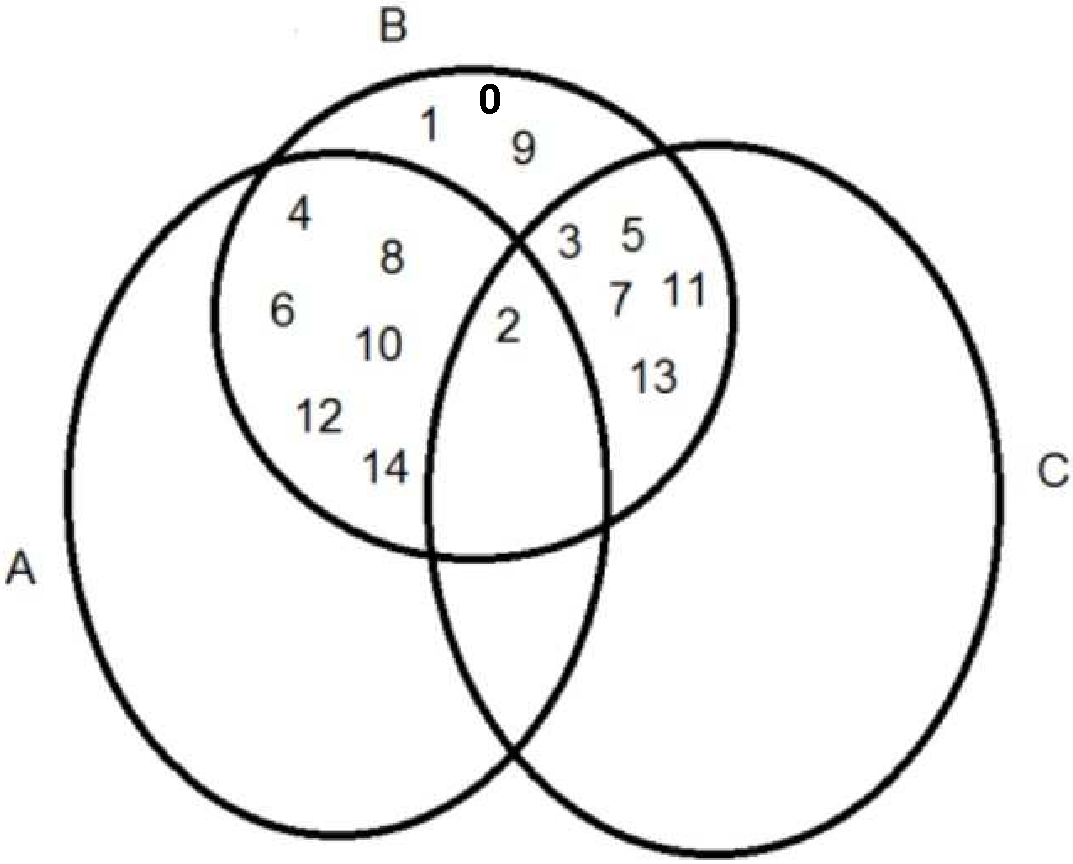
\includegraphics[width=.4\linewidth]{Figs/conjuntos-cropped.pdf}
    \end{center}

\end{Gabarito}
\begin{Gabarito}{18}
~

    \begin{center}
        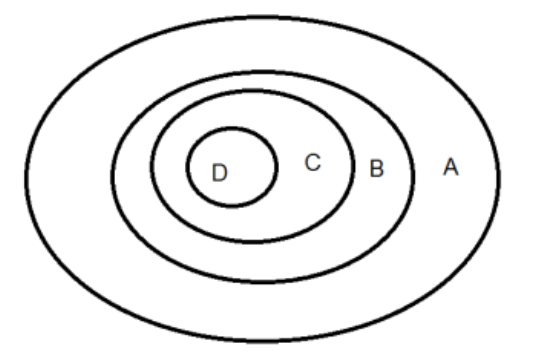
\includegraphics[width=.4\linewidth]{Figs/conjuntos2.png}
    \end{center}
\end{Gabarito}
\begin{Gabarito}{19}
~

    \begin{multicols}{2}
    \begin{enumerate}[a)]
        \item $\{1,2,3,4,5\}$
        \item $\{1,3\}$
        \item $\{5,7,9,11,...\}$
        \item $\{0,5,6,7,8,9,11,13,15,17,...\}$
        \item $\{ 4, 2, \infty\}$
    \end{enumerate}
\end{multicols}

\end{Gabarito}
\begin{Gabarito}{20}
~

    \begin{enumerate}[a)]
        \item $\{(a,x),(a,y),(b,x),(b,y),(c,x),(c,y)\}$
        \item $\{(0,a),(0,b),(0,c),(1,a),(1,b),(1,c)\}$
    \end{enumerate}
\end{Gabarito}
\begin{Gabarito}{21}
~

    \begin{enumerate}[a)]
    \item
    \begin{multicols}{2}
        \begin{itemize}
            \item $A \cup (B \cap \overline{B})$
            \item $A \cup \emptyset$
            \item $A$
        \end{itemize}

        \begin{itemize}
            \item (distributividade)
            \item (complemento)
            \item (elemento neutro)
        \end{itemize}
    \end{multicols}

    \item

    Correção: $A \cap (B \cup \overline{A}) = B \cap A$

    \begin{multicols}{2}
        \begin{itemize}
            \item $(A \cap B) \cup (A \cap \overline{A})$
            \item $(A \cap B) \cup \emptyset$
            \item $(A \cap B)$
            \item $(B \cap A)$
        \end{itemize}

        \begin{itemize}
            \item (distributividade)
            \item (complemento)
            \item (elemento neutro)
            \item (comutatividade)
        \end{itemize}
    \end{multicols}
\end{enumerate}
\end{Gabarito}
\begin{Gabarito}{22}
~

    $A=\{1,3,5,6,7,8,9\}$ e $B=\{2,3,6,9,10\}$
\end{Gabarito}
\begin{Gabarito}{23}
~

    $X=\{1,3,5\}$
\end{Gabarito}
\begin{Gabarito}{24}
~


    a
\end{Gabarito}
 %imprime as soluções
\end{document}
